\documentclass[12pt]{report}

\usepackage{geometry}
\usepackage{tabu}
\usepackage{dirtytalk}
\usepackage{graphicx}
\usepackage{url}
\usepackage{float}
\usepackage{listings}
\usepackage{algpseudocode}
\usepackage{algorithm}
\usepackage{algorithmicx}
\usepackage{subcaption}
\usepackage{verbatim}
\usepackage{amsmath}
\usepackage{wrapfig}
\usepackage{color}

\usepackage{amsthm}
\usepackage{verbatimbox}
\usepackage{multicol}
\usepackage{multirow}
\usepackage[titletoc,title]{appendix}
\usepackage{amsfonts}
\usepackage[font={it}]{caption}
\usepackage{afterpage}
\usepackage{caption}
\usepackage{lipsum}
\usepackage{csquotes}
\usepackage{fancyvrb}
\usepackage{cprotect}
\usepackage[table]{xcolor}

\usepackage{lmodern}

% For citing and referencing.
\usepackage{natbib}
\newcommand{\citebu}[1]{(\citenoparen{#1})}
\newcommand{\citenoparen}[1]{\citeauthor{#1} \citeyear{#1}}
\newcommand{\citediagram}[2]{(\citeauthor{#1} \citeyear{#1}, p.#2)}
\newcommand{\citesoftware}[1]{(\citeauthor{#1} \citeyear{#1})}

\newcommand{\figurewidth}{0.55\textwidth}
\newcommand{\imagewidth}{0.47\textwidth}

\newcommand{\cpp}{C\texttt{++}}
\newcommand{\bgcell}{\cellcolor{lightgray}}

\newcommand{\quotebu}[2]
{
  \begin{displayquote}[\citenoparen{#2}]
    \textit{#1}
  \end{displayquote}
}

\geometry{
  a4paper,
  total={170mm,257mm},
  left=30mm,
  right=30mm,
  top=20mm,
  bottom=30mm,
}

\pagenumbering{roman}

\theoremstyle{definition}
\newtheorem{definition}{Definition}[section]

\begin{document}

  \renewcommand{\familydefault}{\sfdefault}
  \fontfamily{lmss}\selectfont

  \begin{titlepage}
    \centering
    {\Huge Bournemouth University\par}
    \vspace{0.5cm}
    {\Large National Centre for Computer Animation\par}
    \vspace{0.5cm}
    {\Large MSc in Computer Animation and Visual Effects\par}
    \vspace{5cm}
    {\huge \bfseries evulkan\par}
    \vspace{0.5cm}
    {\Large \bfseries \textit{A Vulkan Library}\par}
    \vspace{2cm}
    {\Large Eimear Crotty\par}
    % \includegraphics[width=0.15\textwidth]{images/MIT.png}\par\vspace{1cm}
    \vfill
    {\Large August 2020}
  \end{titlepage}

  \chapter*{Abstract}
    Vulkan is a low-level graphics API which aims to provide users with faster
    draw speeds by removing overhead from the driver. The user is expected to
    explicitly provide the details previously generated by the driver. The
    resulting extra code can be difficult to understand and taxing to write
    for beginners, leading to the need for a helper library.

  \chapter*{Acknowledgements}

    \vspace{1cm}
    Thanks to Jon Macey for his help on the \cpp{} side of things and for loaning
    me his Vulkan book.\\
    
    Many thanks to my uncle Neil for giving me a second home during the year. Those curries
    and trips to the Glasshouse kept me going through multiple challenging assignments.
    I'm sorry they were cut short. \\

    Finally, thanks to my mum Kerry, dad Owen, siblings Rory, Aisling, Aoife and Ellie for
    their support during the last year. \\

  \tableofcontents

  \listoffigures

  \chapter{Introduction}
    \pagenumbering{arabic}
    Vulkan \citesoftware{vulkan} is a cross-platform graphics and compute API.
    It aims to provide higher efficiency than other current
    cross-platform APIs, by using the full performance available in today's
    largely-multithreaded machines. Vulkan achieves this by allowing tasks to be
    generated and submitted to the GPU in parallel (multithreaded programming).
    In addition, the API itself is written at a lower-level than other graphics
    APIs, meaning that the developer is required to provide many of the details
    previously generated by the driver at run-time.\\

    This project aims to alleviate this cost by providing a wrapper library for
    Vulkan, which allows a developer to use some of the more common features of
    Vulkan with much less effort than writing an application from scratch. This
    library is written in \cpp, using modern \cpp features, adheres to both the
    official \cpp Core Guidelines and Google \cpp Style Guide and is fully unit
    tested. The library is available for download from GitHub and can be built
    using CMake.\\

    The library is specifically written with beginners and casual users of
    Vulkan in mind. The examples included in the repository provide a
    demonstration of how to use the library for different purposes, including
    drawing a triangle, loading an OBJ with a texture and using multiple passes
    to render simple objects with deferred shading. A non-goal is to create a
    library which is as fast as writing pure Vulkan, however the library
    must be reasonably fast.\\

  \chapter{Previous Work}

    While Vulkan is a relatively new API for graphics and compute, many engines
    now support Vulkan, including CryEngine, Valve's Source, Unity and Unreal
    Engine. As a result, there are many libraries and utilities available
    online for Vulkan, each of which serves a different purpose.

    \section{V-EZ}

      AMD created the open-source V-EZ library \citesoftware{vez}. Its goal is to increase the
      adoption of Vulkan in the games industry by reducing the complexity of
      Vulkan. It is a lightweight C API wrapped around the basic Vulkan API.
      It is part of the GPU-Open initiative. \\
      
      It still requires the user to have a good knowledge of Vulkan, making it
      difficult for beginners to adopt. For example, some rather complex
      components include semaphores, swapchain creation and lengthy
      enumerations such as

        \begin{figure}[h!]
        \centering
        \verb|VK_BUFFER_USAGE_TRANSFER_DST_BIT|
        \end{figure}

      While it does remove some of the boilerplate, it is still relatively low
      level and, as a result, is not perfectly suited to beginners.

    \section{Anvil}

      The goal of Anvil is to reduce the amount of time taken to write Vulkan
      applications. It is ideal for rapidly prototyping Vulkan applications,
      but it still requires a large amount of writing. It is stated in the
      documentation itself that Anvil is not suitable for beginners.

      \quotebu{
        Anvil is not the right choice for developers who do not have a
        reasonable understanding of how Vulkan works.
      }{anvil}

    \section{GLOVE}

      GLOVE \citesoftware{glove} provides an intermediate layer
      between an OpenGL ES application and Vulkan. It is easy to build and
      integrate new features and has a GL interface for developing applications.

      GLOVE is useful for developing Vulkan applications for embedded devices,
      especially for developers who already have an understanding of GL
      applications. However, GLOVE is not useful for learning Vulkan
      as it only provides a GL interface.

    \section{MoltenVK}

      As Apple hardware lacks native Vulkan driver support, MoltenVK
      \citesoftware{moltenvk} provides an interface over Apple's Metal graphics framework. This provides no
      speedup in terms of development time, it simply allows Vulkan to
      be developed and run on macOS. As a result, it does not provide any
      extra help for beginners to Vulkan.

    \section{Personal Inquiry}

      This library was developed using a previous project as a starting point \citebu{personalinquiry}.
      The base project can be found at http://github.com/eimearc/vulkan.
      It provided the boilerplate to run an instance of Vulkan and it
      saved days of typing 1000 lines of code to simply have a
      starting point. All class construction, library design
      and testing was implemented in this masters project.

  \chapter{Technical Background}

    \section{Useful Resources}

      As Vulkan is a relatively complex topic, many resources, both online and
      in-print, came in useful during this project and may help the reader
      with their Vulkan understanding.

      \begin{itemize}
        \item Vulkan Programming Guide \citebu{vulkanbook}
        \item Sascha Willem's Vulkan examples \citebu{sascha}
        \item Vulkan Tutorial \citebu{vulkantutorial}
        \item ARM Vulkan tutorial \citebu{arm}
      \end{itemize}

    \section{Comparison with OpenGL}

      Vulkan is a low-overhead, cross-platform graphics and computing API.
      It was developed to allow higher performance and more balanced CPU/GPU
      usage in comparison to older APIs such as OpenGL. \\

      \begin{figure}[h]
        \centering
        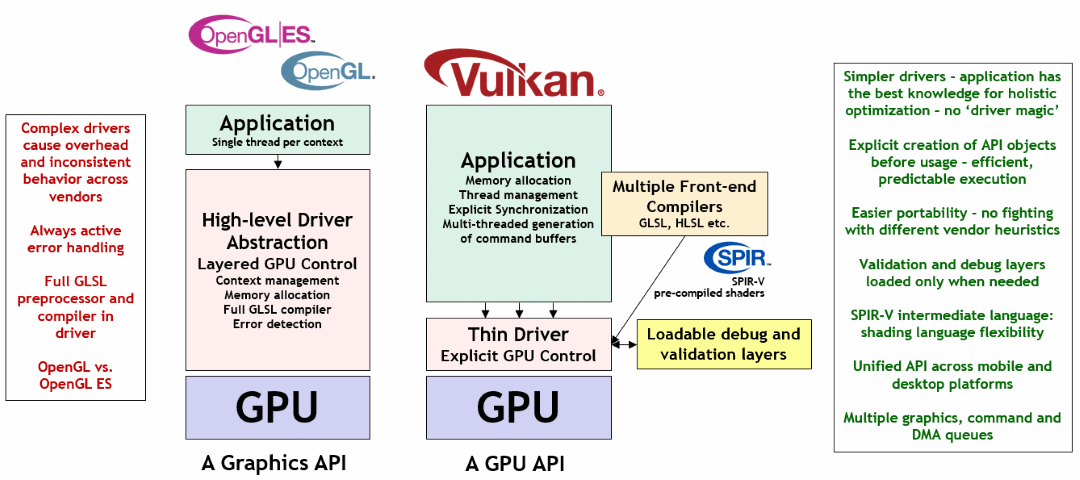
\includegraphics[width=\textwidth]{images/compare_opengl.png}
        \caption{OpenGL compared to Vulkan \citediagram{vulkan_guide}{1}.}
        \label{fig:compare_opengl}  
      \end{figure}

      While OpenGL acts as a state machine, keeping track of application state,
      Vulkan requires the developer to keep track of such state. OpenGL requires
      operations to be submitted in sequence, while Vulkan takes full advantage
      of modern multicore machines and allows operations to be recorded and
      submitted in parallel. \\

      OpenGL handles host-device synchronization and memory management in the
      driver, while Vulkan requires the developer to deal with this. The idea
      behind this is that the developer knows best how their data will be
      accessed and, as a result, the developer knows the optimal way to lay out
      data in memory. While this does result in a more explicit, low level API
      and longer development times, the advantage becomes apparent in the
      runtime speedup. There is much less overhead in the Vulkan driver, as the
      developer provides most of the required detail. Less driver work
      generally results in faster run times. \\

      OpenGL provides a constant level of error checking. While this is useful
      during the development phase, once an application is rolled out to
      production, error checking slows down the application. Vulkan provides
      a way around this with validation layers that can be registered during
      development and removed afterwards, further speeding up an application. \\

      OpenGL reads shader code in GLSL and compiles it at run time. This leads
      to a slower run time in the best case, or run time errors in the worst
      case when the GLSL is not properly formed. Vulkan requires the developer
      to compile the shader code to byte code (SPIR-V) ahead of time and to
      provide as such. This has the dual advantage of ensuring the shader
      code is correct and speeding up the run time. \\

      The pattern is apparent; Vulkan requires more setup, state tracking and
      memory management from the developer. This removes much of the required
      word from the driver, resulting in faster draw speeds in comparison
      with older APIs such as OpenGL.

    \section{Vulkan Layers}

      More traditional APIs have a flat structure. Any calls made to the API are
      forwarded to the driver for more work. If a developer wants to extend the
      structure and capabilities of the API, they are required to either "hack"
      together a platform-specific implementation, or have their extension
      built directly by the API developers into the API and driver. This
      increases the bulkiness of the API, requiring all users to have
      this large API when they may only use the minimal number of features.
      This "all-or-nothing" approach decreases the speed of the application,
      which is quite important for smaller applications running on embedded
      systems. \\

      Vulkan, in contrast, is a layered API, using a loader to create this
      layered architecture. This layered approach results in faster
      applications, as certain features which are needed in development,
      such as validation, can be unloaded when releasing an application.

      \subsection{Loader}

      The Vulkan loader is "the central arbiter in the Vulkan runtime" \citebu{renderdoc}.
      The application interfaces with the loader and it is the task of the
      loader to dispatch incoming requests to the correct subsystem. The
      loader exposes all of the core Vulkan functions. When an application
      calls such functions, they are routed through the loader, instead of
      directly to the driver. \\

      When creating an instance, certain extensions are required. Extensions
      are grouped into layers. These layers are specific to a system and
      platform and are registered in a well-known location on that machine
      in JSON files. These files contain the names of the extensions provided
      by the layer and where to find the actual library is on the system This
      means that whenever the Vulkan loader queries for a specific layer, the
      JSON file is read - the layer module itself does not need to be loaded. \\

      For example, a layer JSON file may be found at \\

      \begin{centering}
        \begin{Verbatim}[fontsize=\small]
/usr/local/share/vulkan/explicit_layer.d/VkLayer_khronos_validation.json
        \end{Verbatim}
      \end{centering}

      Included in the file may be the following (edited for brevity):

      \begin{centering}
        \begin{Verbatim}[fontsize=\small]
"instance_extensions": [
...
  {   
    "spec_version": "1", 
    "name": "VK_EXT_debug_utils"
  },
...
],
...
"library_path": "../../../lib/libVkLayer_khronos_validation.dylib"
        \end{Verbatim}
      \end{centering}


      \subsection{Dispatch Chains}

      A dispatch chain (figure \ref{fig:loader1}) is the path along which execution flows. The application
      calls a function, for example \verb|vkCreateInstance|. In the loader code, the
      layers and extensions are validated. The loader then passes execution
      along to the first layer, which also calls \verb|vkCreateInstance|, then
      passing execution along to the following layer. The loader terminates
      with its own code, before passing off the execution to the ICD
      (installable client driver). All available drivers are now combined
      into one unified front.

      \begin{figure}[h]
        \centering
        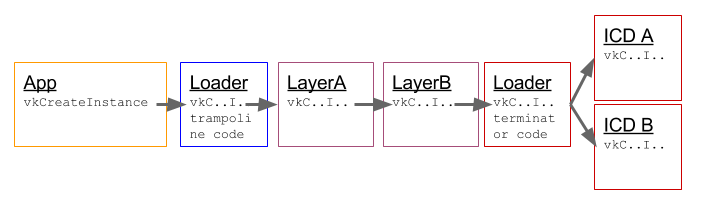
\includegraphics[width=\textwidth]{images/loader1.png}
        \caption{Vulkan dispatch chain \citediagram{renderdoc}{1}.}
        \label{fig:loader1}  
      \end{figure}

      This execution style also creates a dispatch table (figure \ref{fig:loader2}), where each layer in
      the queue calls \verb|vkGetInstanceProcAddr| on the next layer. This long
      chain of function pointers means that each layer knows how to pass on
      control to the next layer in the chain. 


      \begin{figure}[h]
        \centering
        \includegraphics[width=\textwidth]{images/loader2.png}
        \caption{Vulkan dispatch table \citediagram{renderdoc}{1}.}
        \label{fig:loader2}  
      \end{figure}

    \section{Vulkan Components}

      \begin{figure}[h]
        \centering
        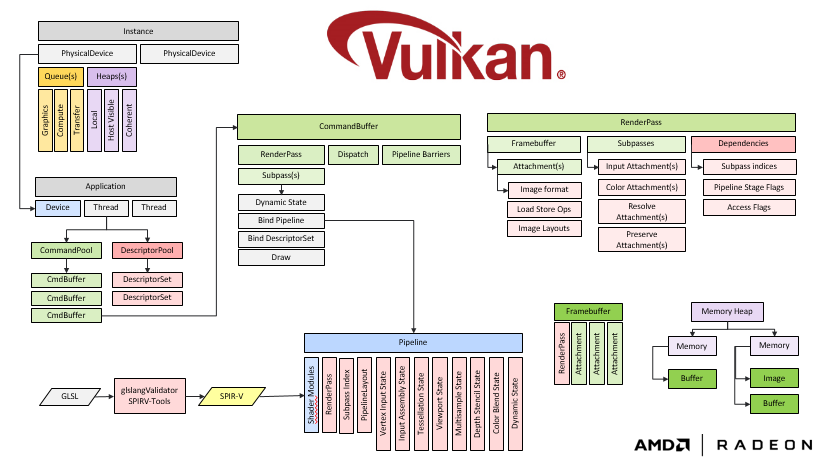
\includegraphics[width=\textwidth]{images/interactions.png}
        \caption{Vulkan API objects and their interactions \citediagram{vez}{1}.}
        \label{fig:interactions}  
      \end{figure}

      \subsection{VkInstance}
      
        A Vulkan instance is the first Vulkan component a developer creates in
        their application.  As Vulkan has no global state, all per-application
        state is contained within a Vulkan instance. By creating a VkInstance,
        the application loads the Vulkan commands and initializes Vulkan.
        Within each instance are multiple physical devices. \\

        After the Vulkan instance is created, devices and queues are the main
        way the application interacts with the Vulkan implementation.

      \subsection{VkPhysicalDevice}

        A physical device represents a single hardware device on the machine
        which has Vulkan capabilities, such as a GPU.

      \subsection{VkDevice}

        A logical device (simply a "device") is a software abstraction around a
        physical device. A physical device is queried for its capabilities and,
        based on required application criteria, a device is created from the
        suitable physical device. A device represents an instance of a
        physical device and contains its own state and resources. This is
        the Vulkan component that is most commonly interacted with and is
        used in constructing all subsequent components. An application is
        required to create a different device for each physical device it uses.
        Each device exposes a number of queues.

      \subsection{VkQueue}

        A queue is where a piece of work is submitted for completion by the GPU,
        for example a draw command. A queue is created in conjunction with a
        device and the application queries the device for a suitable queue.
        Queues are partitioned into a set of families, where each family
        supports one or more types of functionality. Examples of such
        functionality include graphics, presentation and compute. For most
        applications, graphics functionality is required to modify the
        incoming vertices and presentation support is required to display
        the resulting images on the screen. 

        Queue submission occurs when work is submitted to a queue using commands
        such as vkQueueSubmit. Such commands specify a set of underlying
        operations which are to be executed by the associated physical
        device. 

        Each queue works asynchronously to other queues, making it suitable for
        multithreaded use.

      \subsection{VkDeviceMemory}

        Memory is explicitly managed by the application. There are two types of
        memory in Vulkan, host memory and device memory. Device local memory is
        physically connected to the device, while host visible memory is
        visible to the host. Each device exposes the types of memory available
        to the application. \\

        When creating a buffer, the user must specify both how the buffer will
        be used and where this buffer will reside. Host-visible memory can be
        accessible by the CPU through the use of the vkMapMemory command, while
        the device-local is the most efficient for GPU access.

      \subsection{VkCommandBuffer}

        The application can control the device through the submission of command
        buffers. Prior to submission, the application records units of work
        into these command buffers. These command buffers may be constructed
        over multiple threads and may be reused multiple times. The command
        buffers are submitted to queues. Command buffers in separate queues
        may execute in parallel, while command buffers in a single queue
        execute in respect to queue submission order. Upon command buffer
        queue submission, control is returned to the application immediately. \\

        There are two different types of command buffers,
        primary command buffers and secondary command buffers.

        \begin{itemize}
          \item A primary command buffer is submitted to a queue for execution.
          It holds references to an array of secondary command buffers.
          \item A secondary command buffer is not submitted to a queue for
          execution. Instead, work is recorded into it and a reference to the
          command buffer is attached to a primary command buffer, along with
          other secondary command buffers. This allows for multiple threads to
          construct multiple secondary command buffers in parallel, attach
          them to a primary command buffer and submit for execution.
        \end{itemize}

        All of this work can be recorded into the buffers ahead of draw time,
        resulting in faster draw speeds.

      \subsection{VkSwapchainKHR}

        The swapchain is an abstraction around a series of images that are presented
        to the screen. One image is presented at a time, but at the same time 
        the application may be writing to another image (double buffering). The
        minimum and maximum number of images in a swapchain is implementation-dependent.
        It is possible to query Vulkan (using the \texttt{vulkaninfo} command)
        to determine the correct number of images to request in a swapchain. For
        many graphics cards, this number is between 2 and 3 inclusive. \\

        The \texttt{KHR} suffix indicates that this is not a core Vulkan object,
        but is provided as part of an extension. This is because Vulkan is platform-agnostic
        and so cannot tie its presentation support to a single window system or presentation engine. \\

        The application acquires an image from the swapchain using the \texttt{vkAcquireNextImageKHR} command
        and releases it for presentation using the \texttt{vkQueuePresentKHR} command.

    \section{Vulkan Object Model}

      Vulkan objects (VkInstance, VkDevice and so on) are represented by
      handles - an abstract reference to a piece of memory that is managed by
      Vulkan. Handles come in two types; dispatchable and non-dispatchable.

      Dispatchable objects consist of a pointer to an opaque type. These
      objects internally hold a dispatch table. This table is used by other
      components of the system to determine what code to execute when the
      application makes calls to Vulkan. Examples of dispatchable objects
      include the VkInstance, VkPhysicalDevice, VkDevice, VkCommandBuffer
      and VkQueue. The first argument to any Vulkan function is a
      dispatchable object. This excludes VkInstance creation, as this
      is the first dispatchable Vulkan object created.

      Non-dispatchable objects are 64-bit integer types which are
      implementation dependent. They either contain a reference to another
      object, or encode information about the object directly. Objects
      created on a specific device are private to that device and cannot
      be used on another device.

  \chapter{The evulkan Library}

    \section{How does it work?}

      The library exposes a number of components, each of which is a wrapper
      around one or more Vulkan objects.

      \subsection{evk::Device}

        \begin{wrapfigure}{l}{\figurewidth}
          \centering
          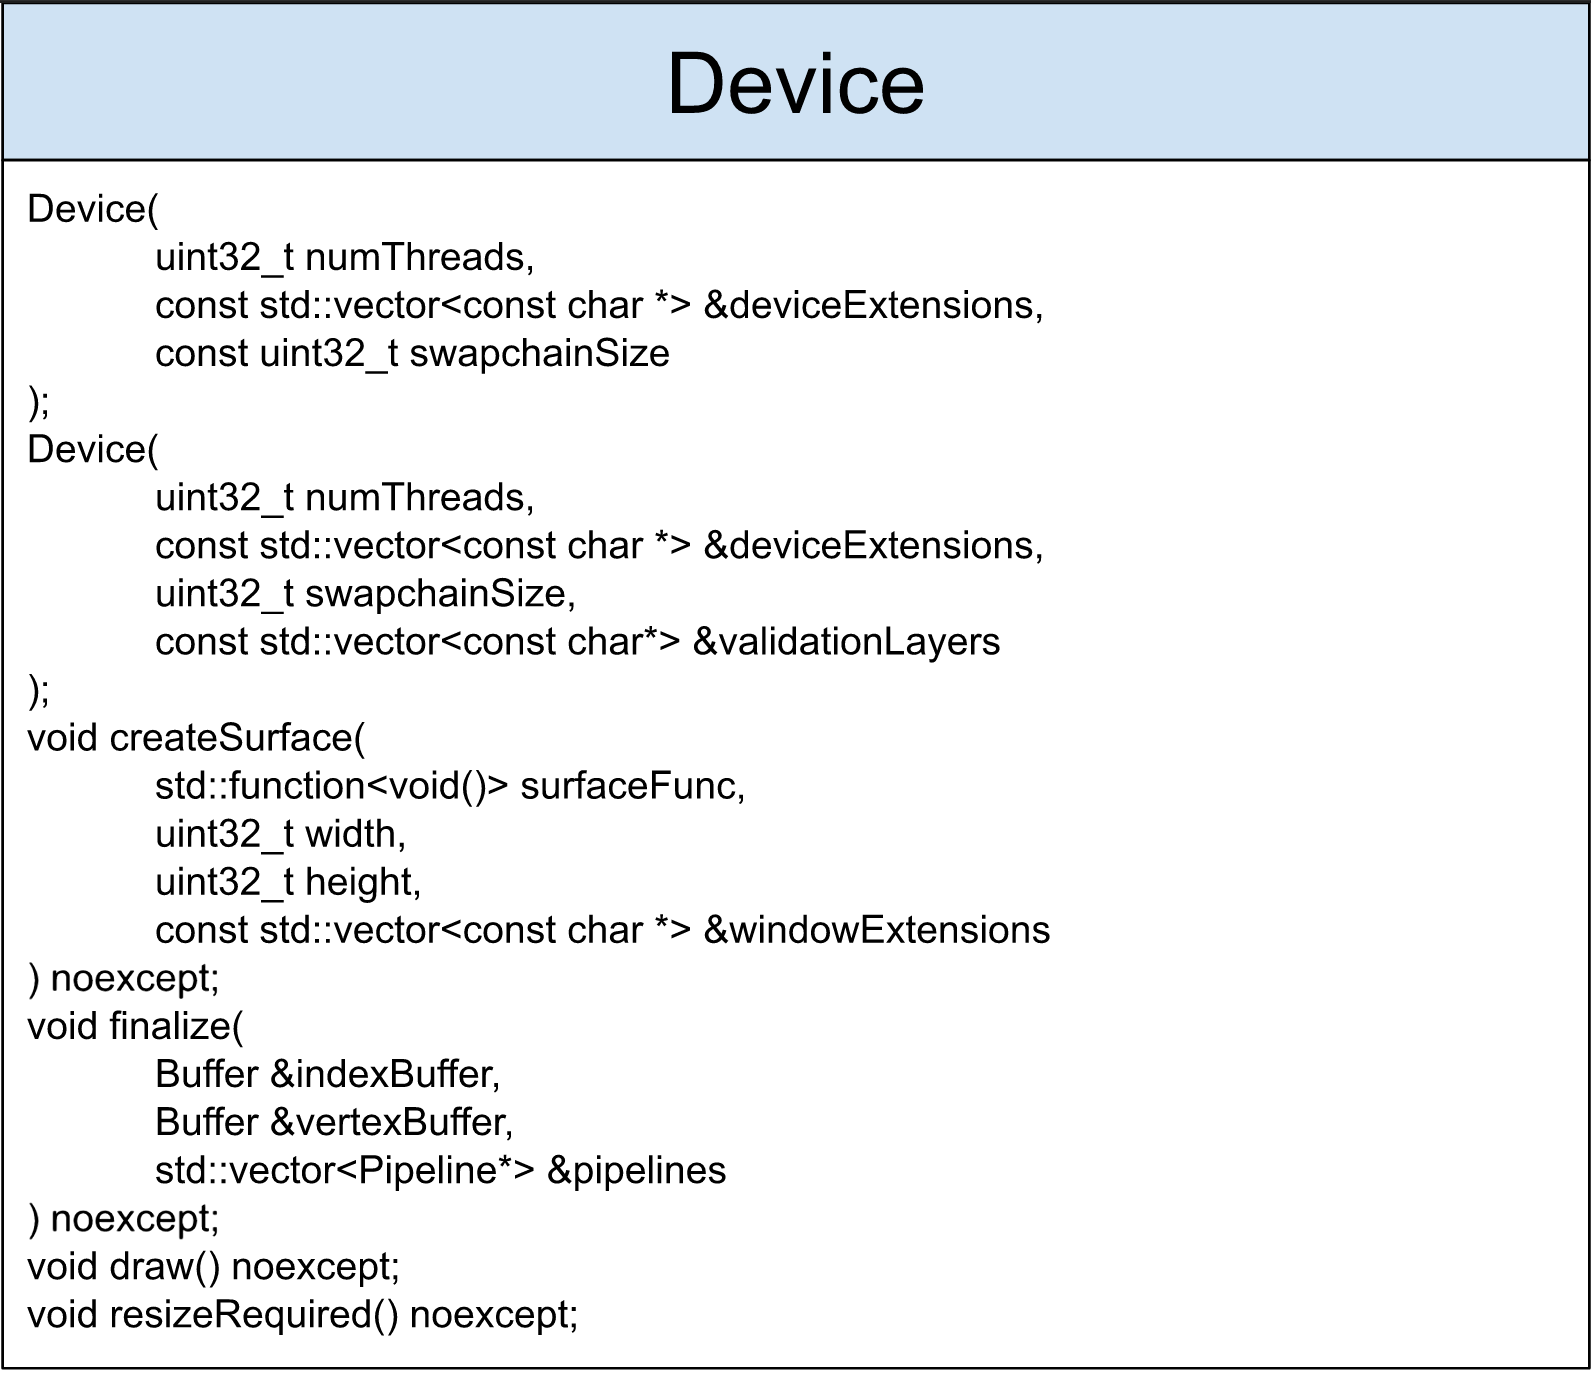
\includegraphics[width=\imagewidth]{images/class_device.png}
          \caption{Device class diagram.}
          \label{fig:class_device}  
        \end{wrapfigure}

        A device is the basic component of the library. It is the first Vulkan
        component that is constructed in the application. It encapsulates,
        among other things, a VkInstance, VkPhysicalDevice, VkDevice, VkQueues.
        A user can set up the device with or without validation layers. Leaving
        validation layers turned off results in a faster application suitable
        for production. \\

        The Device object tracks state across the program. It is used in the
        creation of other evk Vulkan objects. The Device is responsible for
        creating a VkInstance, VkPhysicalDevice, VkDevice, VkSwapchainKHR, VkFramebuffer
        and all the required command buffers. \\

        The Device is multithreaded, making use of Vulkan's multithreading
        capabilities. For some more intensive operations, such as recording
        draw operations into the command buffer, it splits the operation
        across multiple threads, each of which records its portion of the
        operation into a separate secondary command buffer. \\

        \begin{figure}[H]
        \begin{verbatim}
            vkCmdDrawIndexed(
              secondaryCommandBuffer, numIndices,
              1, indexOffset, 0, 0
            );
        \end{verbatim}
        \end{figure}

        These secondary command buffers are then executed from the primary
        command buffer.

        \begin{figure}[H]
        \begin{verbatim}
            vkCmdExecuteCommands(
              primaryCommandBuffer,
              secondaryCommandBuffers.size(),
              secondaryCommandBuffers.data()
            );
        \end{verbatim}
        \end{figure}

      \subsection{evk::Texture}

        \begin{wrapfigure}{r}{\figurewidth}
          \centering
          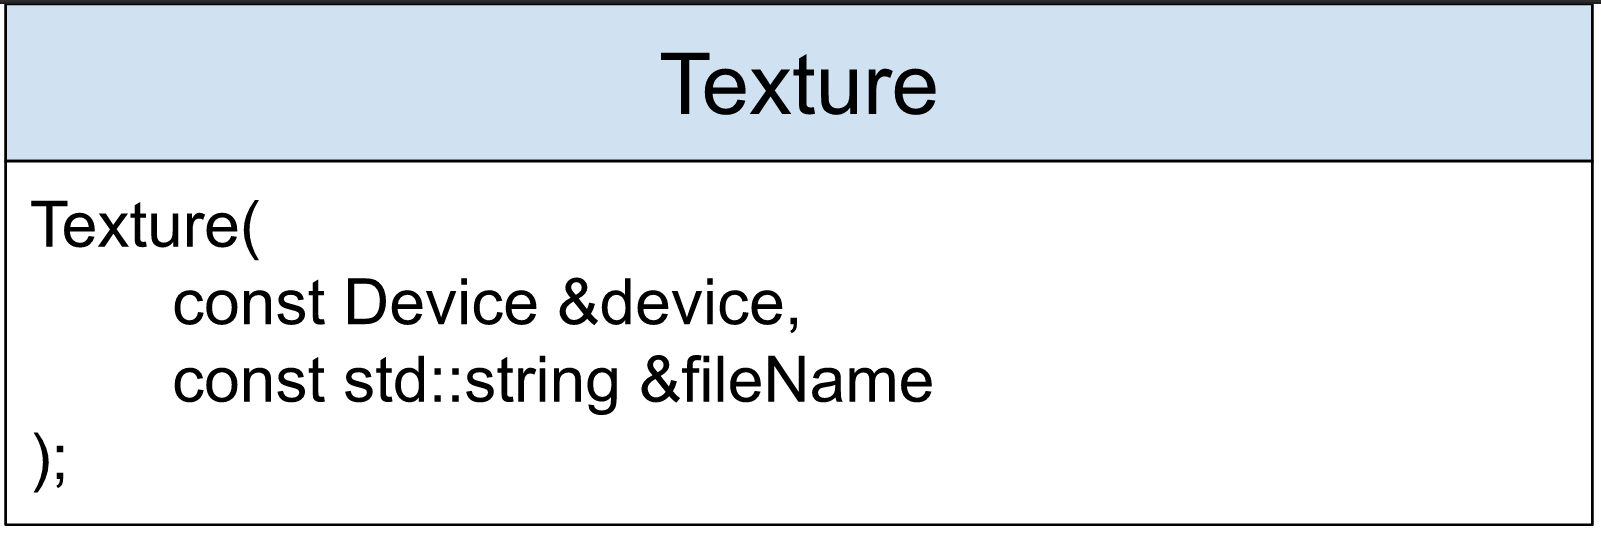
\includegraphics[width=\imagewidth]{images/class_texture.png}
          \caption{Texture class diagram.}
          \label{fig:class_texture}  
        \end{wrapfigure}

        A Texture allows a user to load in a texture from a file. It transitions
        the image to a transfer-optimal format before copying the pixels from
        the image to device-local memory, allowing for faster GPU access. It
        then transitions the image to a layout readable by the shader, frees
        unneeded resources and finally creates a VkImageView and VkSampler. \\

        A VkImageView is required by the Shaders to access images. They
        represent contiguous ranges of subresources and any metadata
        required to operate on them. A VkSampler is a handle to an image
        sampler and is used by the Shader to read image data from Textures
        and apply filters.

      \subsection{evk::Attachment}

        An Attachment represents a resource that can be read from, or written
        to by a Shader. Each Attachment has a binding location and a Type, one
        of FRAMEBUFFER, COLOR or DEPTH. Both a FRAMEBUFFER and DEPTH Attachment
        are required for any program as the shaders must write to the depth
        buffer and to the screen. For more advanced usages (see the multipass
        example) a COLOR Attachment is useful. \\

        An Attachment consists of a VkAttachmentDescription, which describes
        the properties of the Attachment, and multiple VkAttachmentReferences,
        which allow other stages to refer to these Attachments. For DEPTH and
        COLOR Attachments, a VkImage is created, while this is already created
        in the Device creation stage for the FRAMEBUFFER Attachment. \\

        An Attachment also contains a VkClearValue. This value specifies how an
        Attachment should be cleared when it is reused. \\

        \begin{wrapfigure}{l}{\figurewidth}
          \centering
          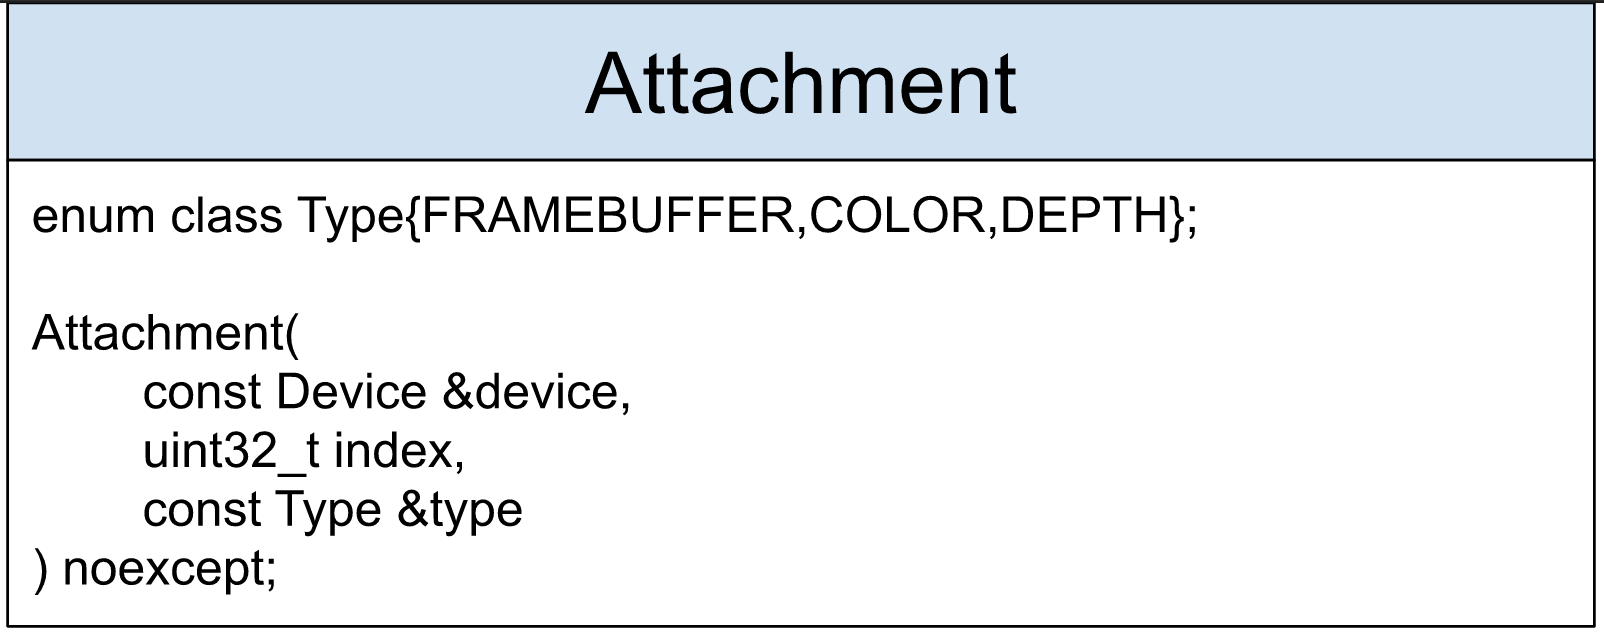
\includegraphics[width=\imagewidth]{images/class_attachment.png}
          \caption{Attachment class diagram.}
          \label{fig:class_attachment}  
        \end{wrapfigure}

        Attachments are used in Subpasses as either an input attachment, a
        colour attachment or a depth attachment. A colour or depth attachment
        is written by the shader, while an input attachment is read into a
        shader, making it useful for multipass rendering.

      \subsection{evk::Buffer}

        A Buffer encapsulates VkBuffer-related structs and methods. It handles
        the creation and copying of VkBuffers, which are linear arrays of
        data, along with copying user data into them and updating them after
        creation. There are two types of Buffers; StaticBuffer and
        DynamicBuffer. \\

        \begin{wrapfigure}{r}{\figurewidth}
          \centering
          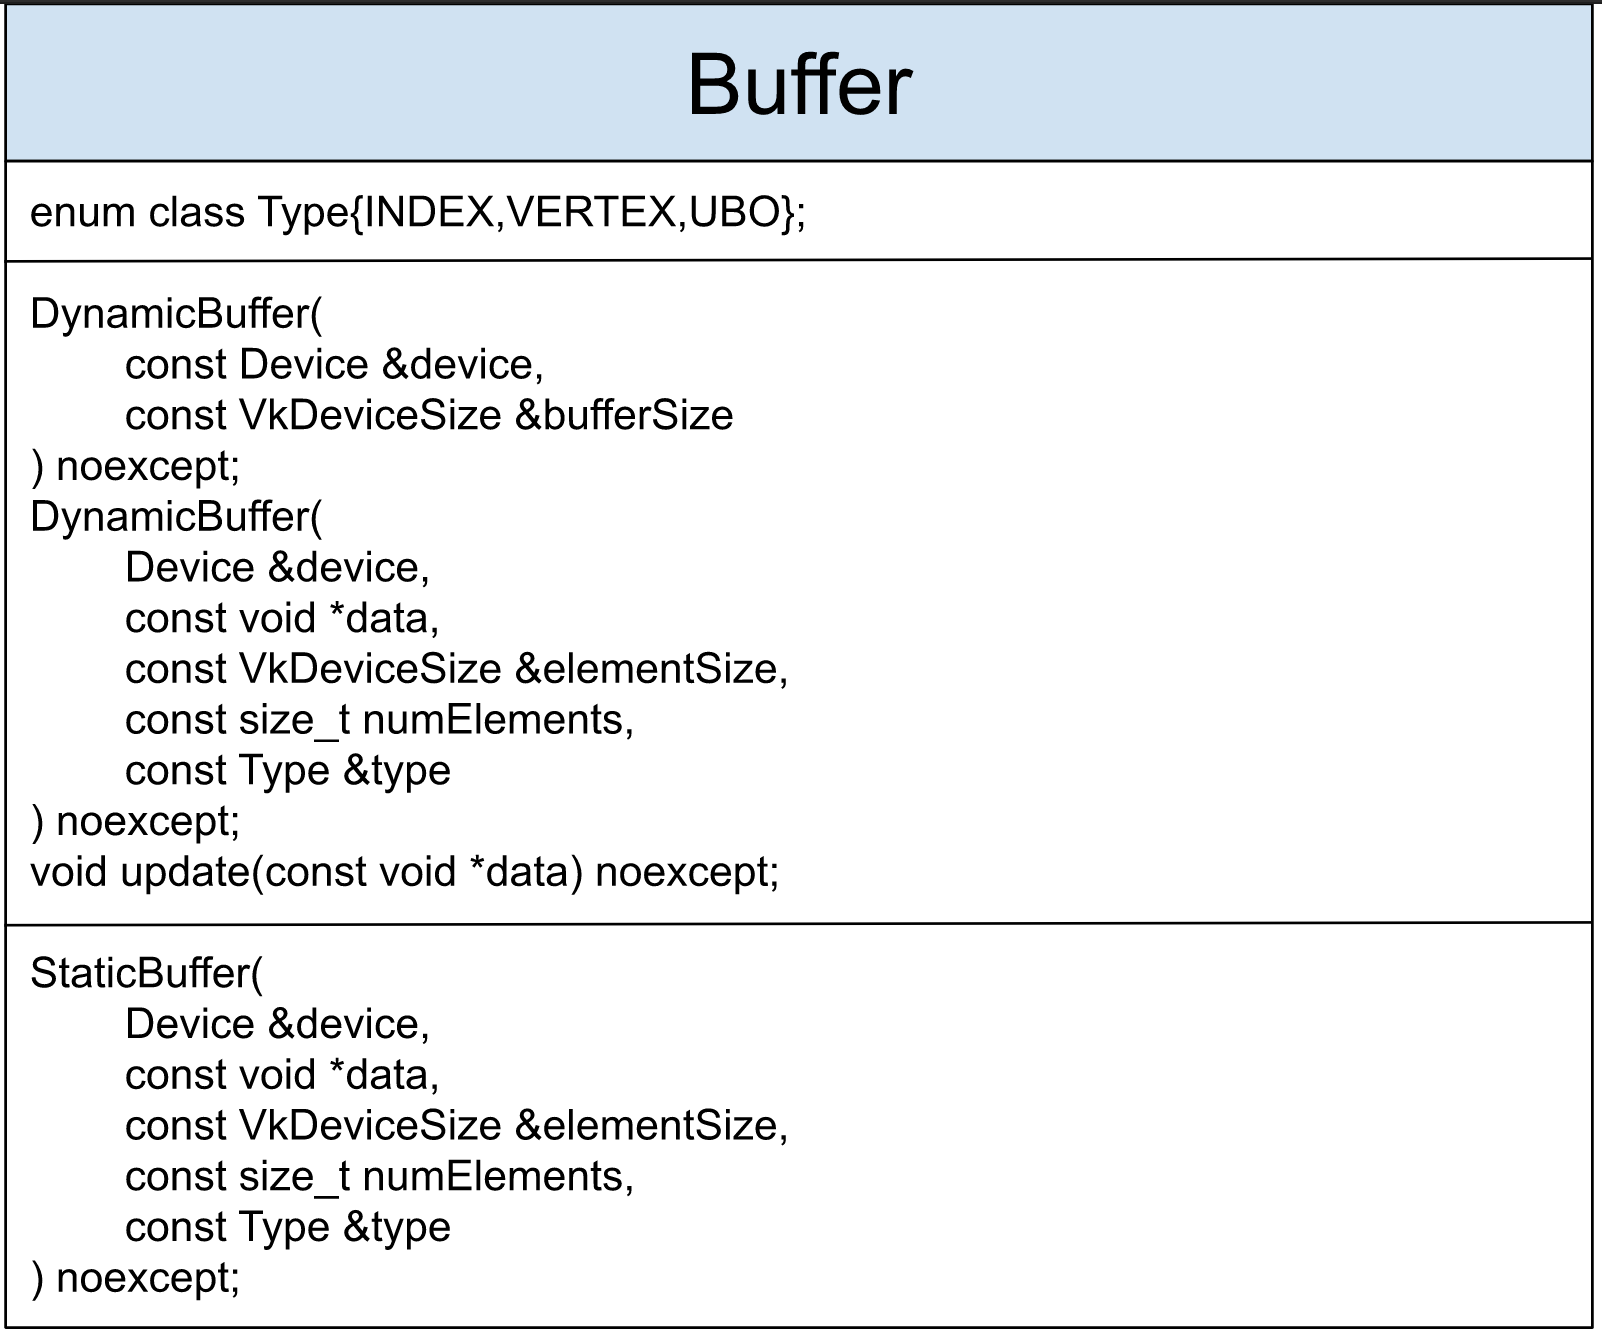
\includegraphics[width=\imagewidth]{images/class_buffer.png}
          \caption{Buffer class diagram.}
          \label{fig:class_buffer}  
        \end{wrapfigure}

        A StaticBuffer is used when the contents of the Buffer will not be
        updated after they have been set. This allows for some optimization
        to take place. The Buffer contents are copied to device-local memory
        to allow faster GPU-access at draw time. \\

        A DynamicBuffer is used when the Buffer contents will be updated at
        draw time. This skips the relatively expensive step of copying the
        Buffer data to device-local memory, and leaves them in host-visible
        memory for faster update speeds. A DynamicBuffer can be updated
        using the update() command.

      \subsection{evk::Descriptor}

        \begin{figure}[h]
          \centering
          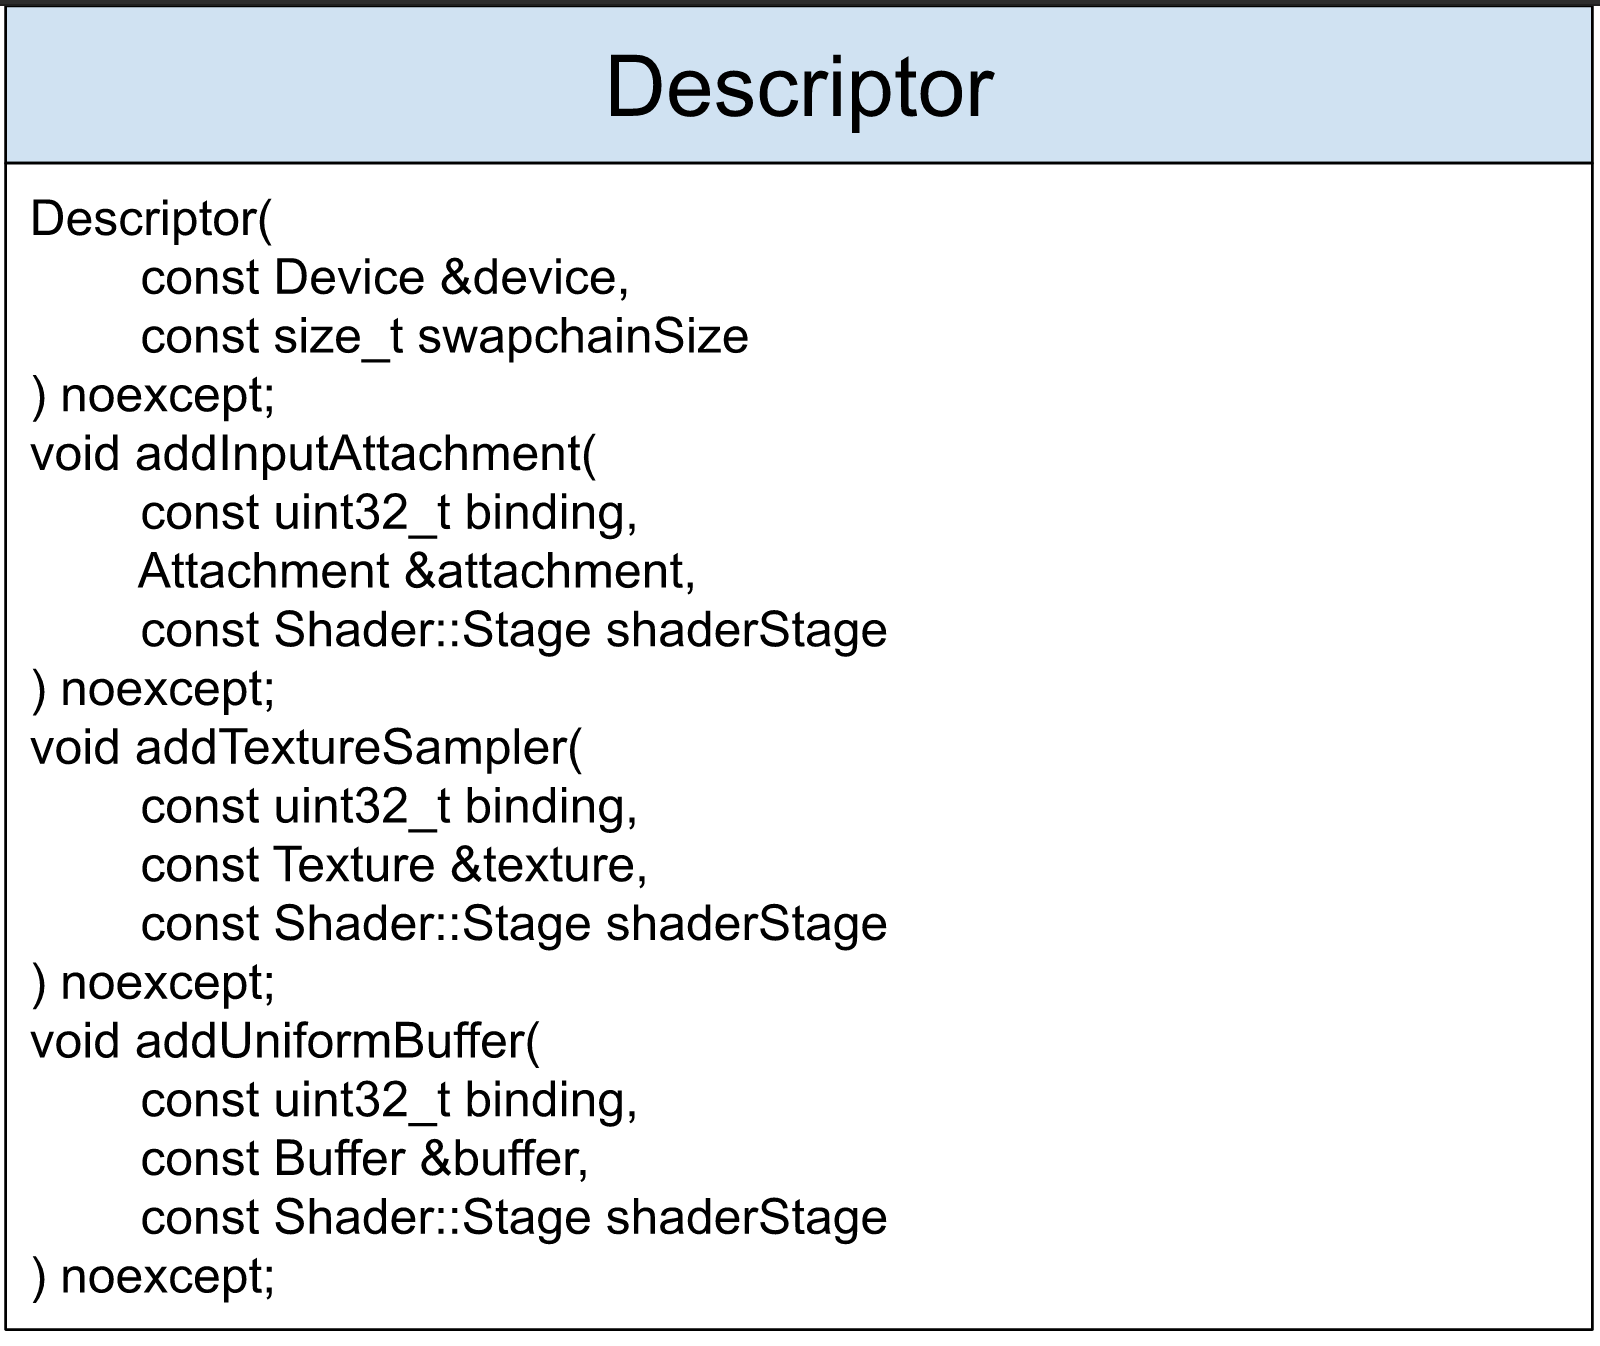
\includegraphics[width=0.35\textwidth]{images/class_descriptor.png}
          \caption{Descriptor class diagram.}
          \label{fig:class_descriptor}
        \end{figure}

        A Descriptor is used to describe any resources that will be accessed by
        the Shader, such as a texture sampler, a uniform buffer or an input
        attachment. A user constructs a Descriptor and then adds the necessary
        resources using class methods. Descriptors are bound in advance of draw
        commands.

        When a user calls one of these functions, for example
        addTextureSampler(), the following happens:

        \begin{itemize}
          \item A VkDescriptorSetLayoutBinding is constructed. This describes
            the shader stage (e.g. a fragment shader) at which the resource
            will be accessed, in addition to the type of the resource.
          \item A VkWriteDescriptorSet is constructed, specifying the binding
            of the resource, along with the type and any other information
            required for a descriptor set write operation. In this example,
            extra information includes the texture sampler handle along with
            the image view handle.
          \item Later on in the program, during pipeline creation, the
            finalize() method is called on the Descriptor. This creates the
            VkDescriptorPool, from which the VkDescriptorSets are allocated.
            VkDescriptorSets are sets of resources which are bound into the
            VkPipeline as a group. Finally, the VkWriteDescriptorSets are
            updated using vkUpdateDescriptorSets() command, binding the
            resources into the descriptor sets.
        \end{itemize}

      \subsection{evk::Subpass}

        \begin{wrapfigure}{l}{\figurewidth}
          \centering
          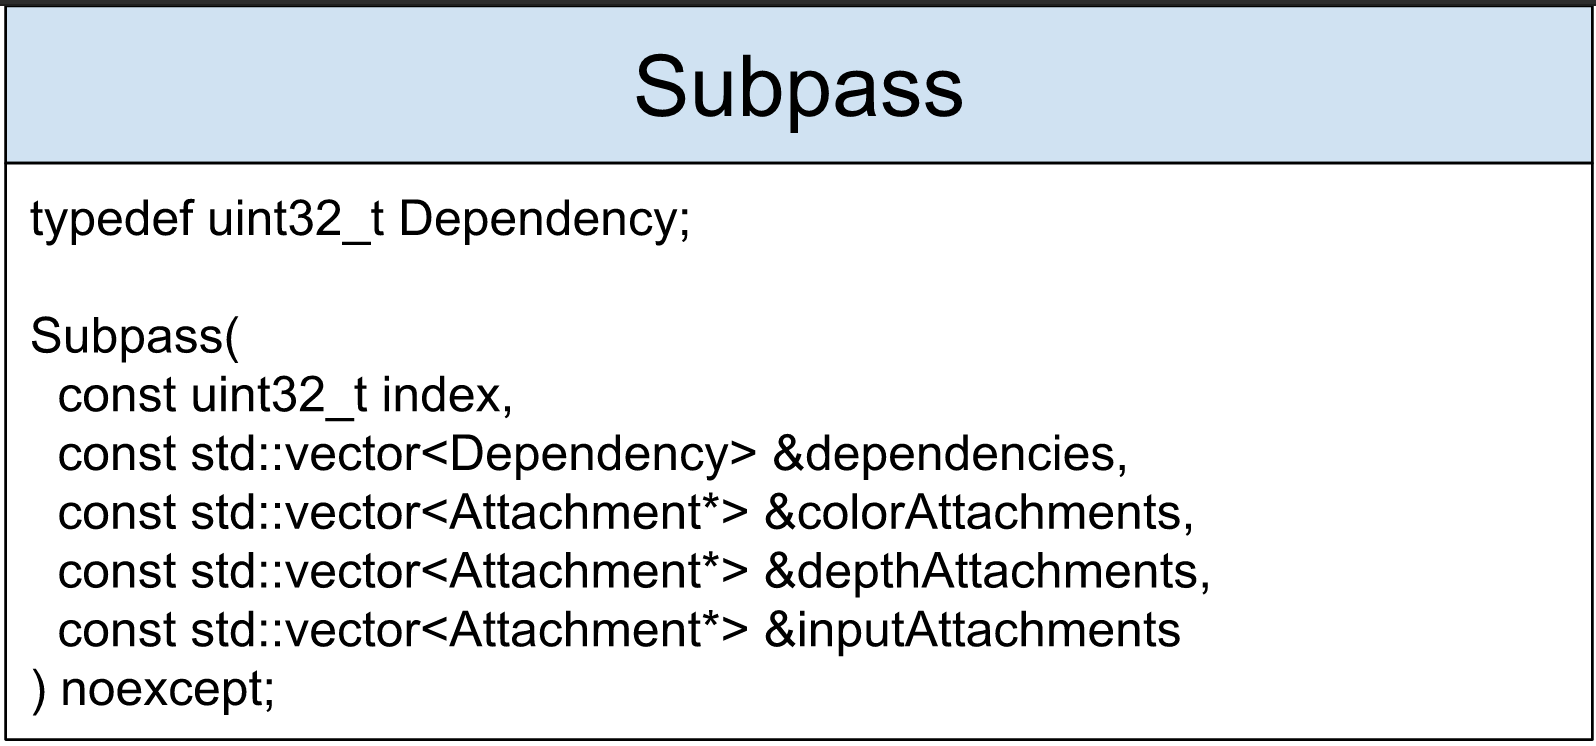
\includegraphics[width=\imagewidth]{images/class_subpass.png}
          \caption{Subpass class diagram.}
          \label{fig:class_subpass}
        \end{wrapfigure}

        A Subpass describes a pass, or a phase of operation, within a
        Renderpass. It can depend on the completion of other Subpasses.
        It has a set of Attachments, which can be either colour, depth or
        input Attachments (as described above) along with their references.
        Contained within the Subpass is a VkSubpassDescription, a struct
        describing the Subpass. The index of the Subpass indicates when the
        Subpass will be executed in order.

      \subsection{evk::Renderpass}

        \begin{wrapfigure}{l}{\figurewidth}
          \centering
          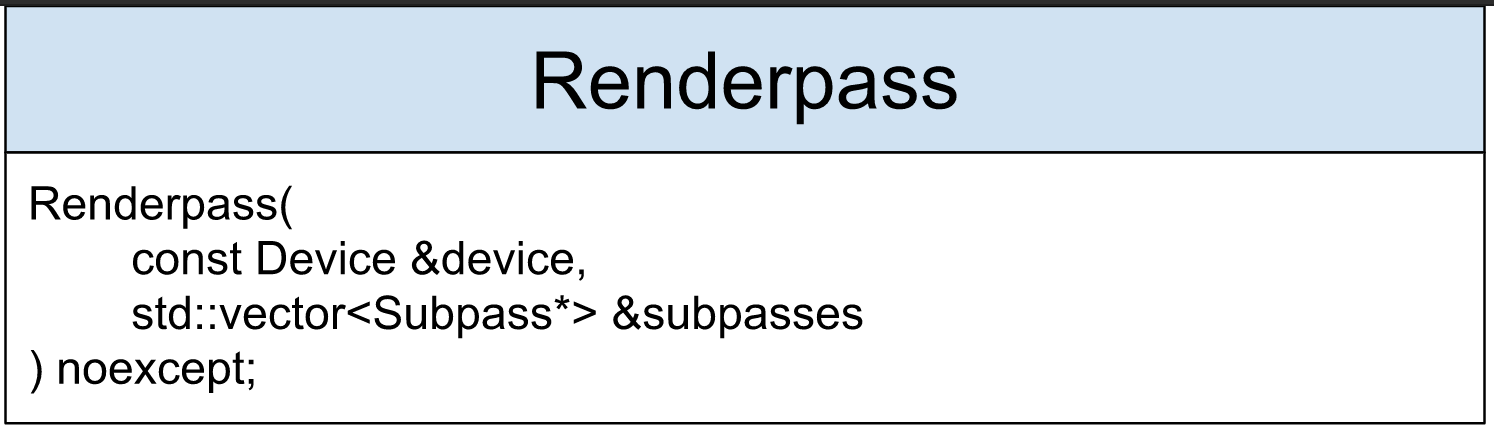
\includegraphics[width=\imagewidth]{images/class_renderpass.png}
          \caption{Renderpass class diagram.}
          \label{fig:class_renderpass}
        \end{wrapfigure}

        A Renderpass object is a collection of Subpasses, along with their
        dependencies and attachments. A VkRenderPass is created within the
        Renderpass by passing in the set of VkSubpassDescriptions,
        VkAttachmentDescriptions and the VkSubpassDependencies between
        subpasses.

      \subsection{evk::Pipeline}

        A Pipeline takes all the previous information and generates a
        VkPipeline - the sequence of operations that take the input vertices
        and produces the output, to the screen or otherwise. We will only
        cover graphics pipeline creation here. A Pipeline is associated with
        exactly one Subpass.
        
        \begin{figure}[h]
          \centering
          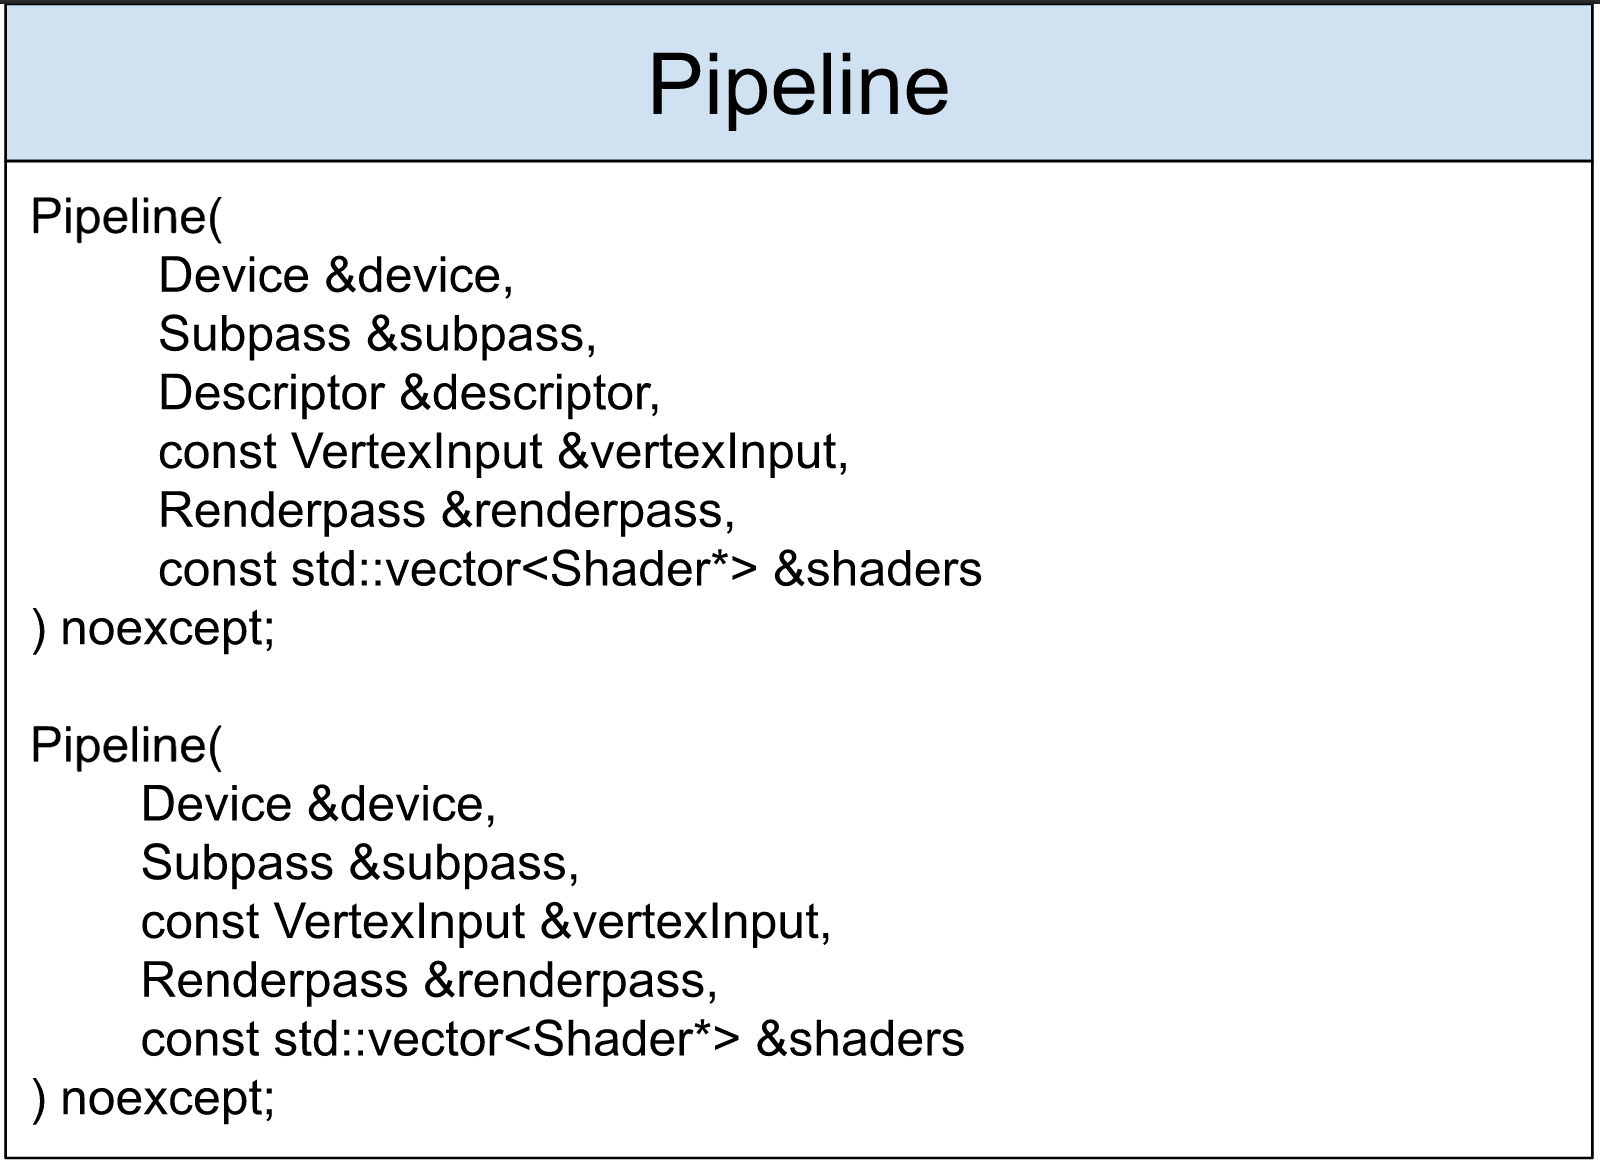
\includegraphics[width=\imagewidth]{images/class_pipeline.png}
          \caption{Pipeline class diagram.}
          \label{fig:class_pipeline}
        \end{figure}

        A Pipeline setup call takes the user-provided Shaders, Renderpass and
        Subpass index, and combines it with automatically generated
        fixed-function information (input assembly, viewport state,
        rasterizer, multisampling, colour blending) to create the VkPipeline.

      \subsection{evk::Shader}

        A Shader represents a shader program, which contains operations that
        execute for each vertex or fragment. A shader contains a
        VkShaderModule, which contains the shader code, and a
        VkPipelineShaderStageCreateInfo struct, which is used during
        Pipeline construction.

        \begin{wrapfigure}{l}{\figurewidth}
          \centering
          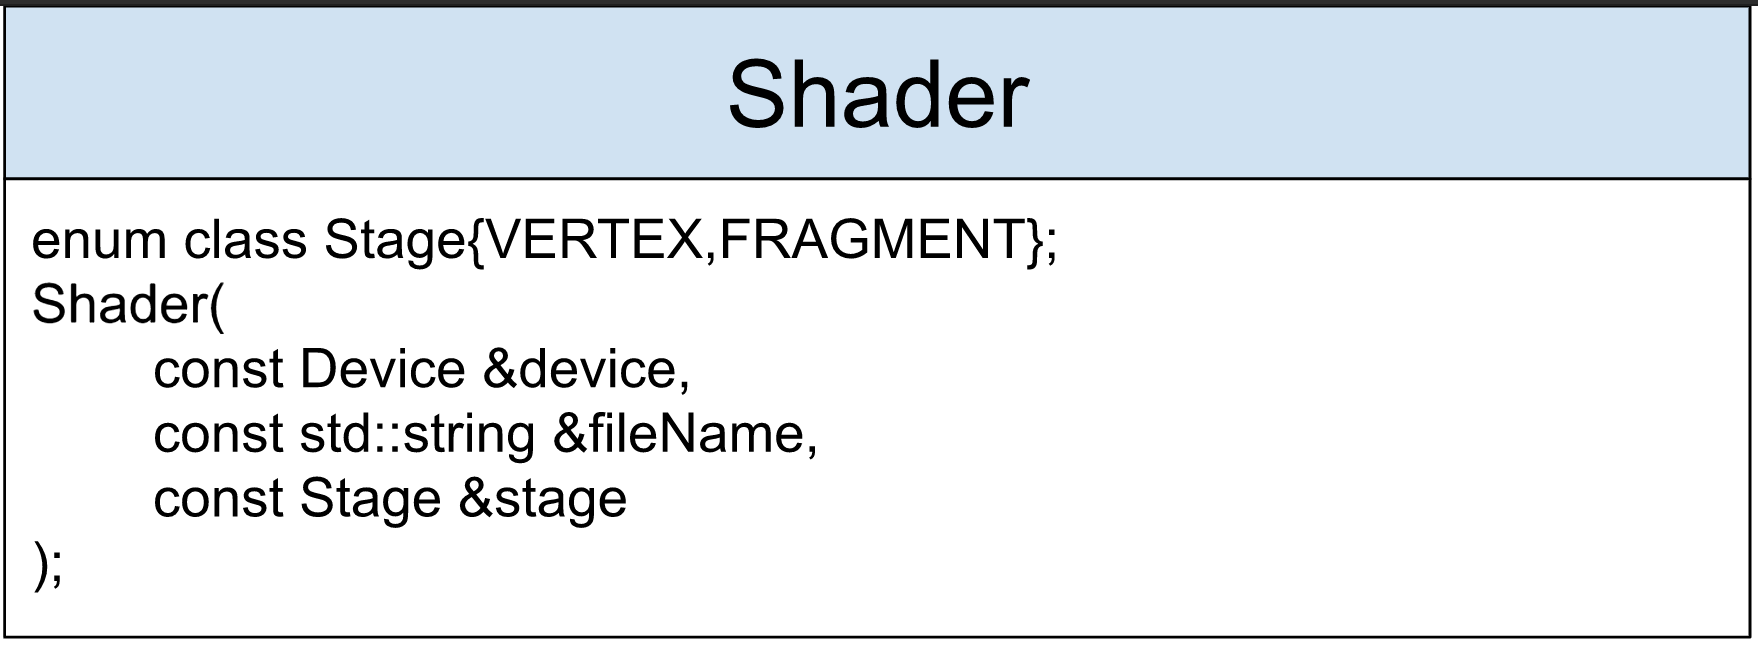
\includegraphics[width=\imagewidth]{images/class_shader.png}
          \caption{Shader class diagram.}
          \label{fig:class_shader}
        \end{wrapfigure}

        There are two supported Shader stages, vertex and fragment. A
        vertex Shader operates on each vertex and any associated vertex
        input attributes, specified using the VertexInput struct. A
        fragment Shader operates on every fragment. Both a vertex Shader
        and fragment Shader are required for the evulkan library.

        A user can load in SPIR-V code from a file of their choice. SPIR-V is
        easily generated from GLSL using the glslc command, which is
        available for download from https://github.com/google/shaderc, or
        with the Vulkan SDK from LunarG.

      \subsection{evk::VertexInput}

        \begin{figure}[h]
          \centering
          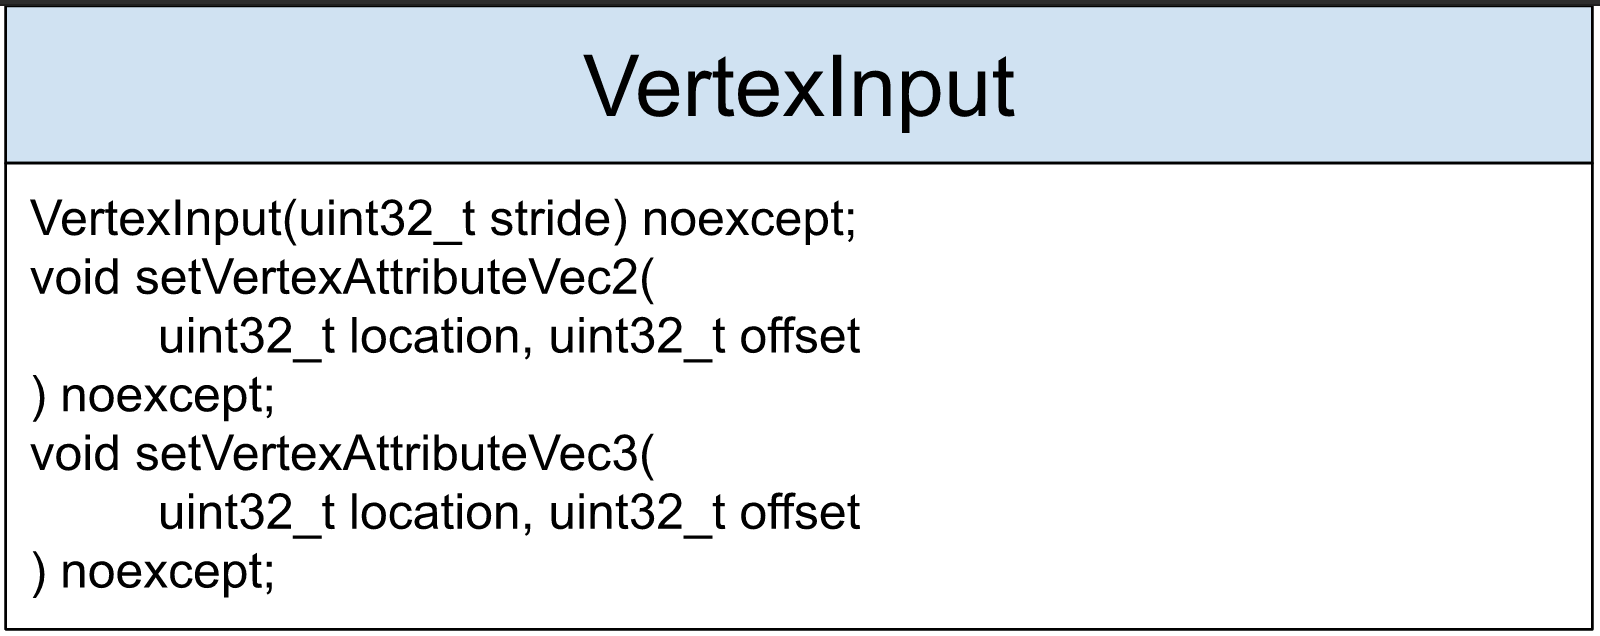
\includegraphics[width=\imagewidth]{images/class_vertexinput.png}
          \caption{VertexInput class diagram.}
          \label{fig:class_vertexinput}
        \end{figure}

        A VertexInput object is a wrapper around a VkVertexInputAttributeDescription
        and a VkVertexInputBindingDescription. It is used for describing vertex
        attributes that will be bound to the shader, such as colour and normal.

      \subsection{Window System Integration}

        Vulkan is a platform-agnostic API. It is up to the application to
        specify the extensions required to interface with the window system.
        The way in which the VkSurfaceKHR object is created also needs to be
        handled by the application. \\

        To keep the evk library platform-agnostic, the user must register
        two things: a function which will be called to create the surface
        and the set of instance extensions required for Vulkan to correctly
        interface with the surface object. For GLFW, this may result in
        something like the following

        \begin{centering}
          \begin{Verbatim}[fontsize=\small]
auto glfwExtensions = glfwGetRequiredInstanceExtensions(
                        &glfwExtensionCount
                      );

std::vector<const char*> surfaceExtensions(
  glfwExtensions, glfwExtensions + glfwExtensionCount
);

auto surfaceFunc = [&](){
  glfwCreateWindowSurface(
    device.instance(), window, nullptr, &device.surface()
  );
};

device.createSurface(surfaceFunc,800,600,surfaceExtensions);
          \end{Verbatim}
        \end{centering}

        For SDL, the following would suffice

        \begin{centering}
          \begin{Verbatim}[fontsize=\small]
SDL_Vulkan_GetInstanceExtensions(
  window, &sdlExtensionCount, surfaceExtensions
);

auto surfaceFunc = [&](){
  SDL_Vulkan_CreateSurface(
    window, device.instance(), &device.surface()
  );
};

device.createSurface(
  surfaceFunc,800,600,surfaceExtensions
);
          \end{Verbatim}
        \end{centering}

          When a window is resized, the evk library automatically recreates the
          required objects (swapchain, framebuffer, input attachments). The
          window resize triggers a \verb|VK_ERROR_OUT_OF_DATE_KHR| or \verb|VK_SUBOPTIMAL_KHR|
          result from either the vkAcquireNextImageKHR() function or the
          vkQueuePresentKHR() function within the draw() method. However,
          there are times when the platform or driver does not correctly
          trigger a resize event. As such, it is recommended that the user register
          a callback function as follows

        \begin{centering}
          \begin{Verbatim}[fontsize=\small]
glfwSetFramebufferSizeCallback(window, framebufferResizeCallback);
          \end{Verbatim}
        \end{centering}

      \subsection{Error Handling}

        Error handling is a contentious topic. Different people have different
        (strong) opinions on which approach to take. Unlike other programming
        languages, \cpp{} does not have a unified approach to error handling,
        leading to diverging dialects of the language. \\

        There are two main types of errors: user errors and programming errors.
        The former are the fault of the person using the library, while the
        latter are the fault of the library developer. User errors should be
        reported to the user and the program should continue execution.
        Programming errors, on the other hand, should halt the program and
        provide as low level information to help the programmer debug the
        issue. Such errors would then be fixed before release (ideally). \\

        \subsubsection{Error Return Codes}

          A common way to handle errors is to return a simple type (bool or int)
          which the user can then test to determine if a method succeeded.

          \begin{figure}[h]
            \centering
            \verb|bool create_file(const std::string &name);|
          \end{figure}

          There are many problems with this approach.

          \begin{itemize}
            \item The return channel is blocked with the error code, meaning
              the function can not return anything else. A solution would be to
              use out parameters.
            \item A bool has low information bandwidth - it tells us if an
              operation failed, but it does not tell us how or why it failed.
              Of course, the bool type could be extended to use an unsigned int,
              but then it is up to the user to compare the int against enums to
              determine the correct path to take. This can be messy. Messy code
              is brittle code.
            \item The user can choose to ignore the value and continue on,
              leading to reduced code safety. A nodiscard keyword could be
              added here, but only if the error is being returned, not used
              as an out parameter as specified above.
            \item The code that is written to handle the error can be totally
              unrelated to the code that detects the error. For example, a
              function 30 levels deep into the call stack might generate an
              error that can only be handled at the top level in main.
          \end{itemize}

        \subsubsection{Exceptions}

          Exceptions are the official way to handle errors. It involves
          throwing an error in the body of code and catching it and dealing
          with it somewhere else.

          \begin{figure}[h]
            \centering
            \begin{verbatim}
void create_file(const std::string &name);

try
{
  create_file("my_file.txt");
} catch(std::exception &e)
{
  // Handle error.
}
            \end{verbatim}
          \end{figure}

          There are some problems with using exceptions:

          \begin{itemize}
            \item Exceptions augment the function stack frame to include
              information about how to handle an exception by unwinding the stack.
            \item Like error codes, there is a disconnect between the code
              that throws the exception and the code that catches the exception.
              There may be functions embedded within the two that become
              involved in the stack unwinding process. Such disconnect makes
              writing robust programs difficult. It means that every part of
              the code needs to be able to handle a less-than-graceful exit.
            \item Again like error codes, the user might have to figure out
              how to handle the plethora of possible exceptions generated by
              the code.
          \end{itemize}

          \quotebu{
            By using exceptions instead of just crashing we are creating a more
            complicated API (the API now includes all the different exceptions
            that the different functions might call) and significantly
            increasing the mental burden on the caller for very little gain.
          }{gamasutra}

          \cpp20 has a proposal in the works for contract-based programming
          which eliminates many of these problems, but as this library is
          explicitly being developed for \cpp14, it's out of scope. \\

          Some developers advocate against the use of exceptions completely,
          disabling their use at the compiler level. Instead, they use
          assertions.

        \subsubsection{Assertions}

          An assertion checks an expression passed to it. If it evaluates to
          true, nothing happens - if it evaluates to false, the program is
          halted and some information is displayed to the developer.
          Assertions can be extended to pass helpful messages to the
          developer. \\

          Assertions ensure that invariants hold. By placing assertions
          throughout a code base, potentially difficult to find bugs manifest
          themselves before they become a problem. The error cannot be ignored
          as the program has crashed. \\

          Assertions are defined using macros and are used during development.
          Prior to release, they can be removed to gain some performance. By
          toggling a variable, assertions can be easily switched on and off. \\

          Assertions are the industry standard for video games, and, as such,
          they are used in the evulkan library. The Game Engine Architecture Book \citebu{gameEngineBook}
          has an excellent section discussing the advantages and disadvantages of
          different kinds of error handling.

      \subsection{Architecture}

        \begin{figure}[h]
          \centering
          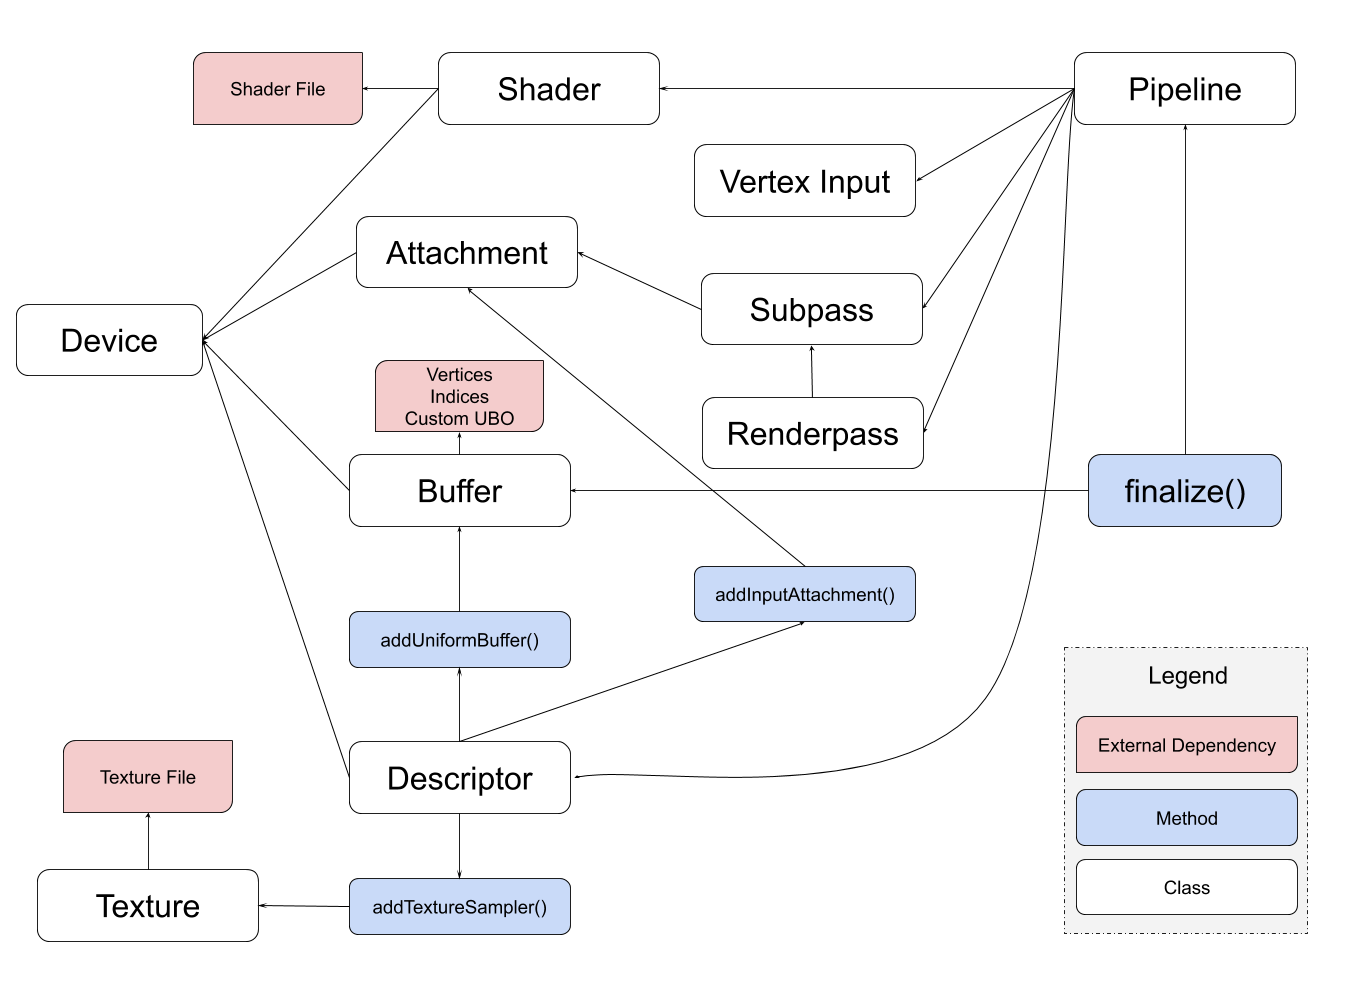
\includegraphics[width=\textwidth]{images/evk_architecture.png}
          \caption{evulkan architecture.}
          \label{fig:evulkan_architecture}  
        \end{figure}

    \section{Installation and Use}

        As the library uses CMake, it is relatively easy to install. Follow
        these instruction in figure \ref{fig:installation} from the root of the directory.

          \begin{figure}
            \centering
            \begin{verbatim}
$ mkdir build
$ cd build
$ cmake ..
$ make
$ make install
            \end{verbatim}
            \caption{instructions for installing evulkan.}
            \label{fig:installation}
          \end{figure}

        The library and header file will be installed in \texttt{/usr/local/} by default.

    \section{Known Problems}

      \subsection{Colo(u)r}

        Spelling is always an issue in writing code, given the wide-reaching
        nature of its collaboration. In order to match the spelling of the
        (mostly American led) Vulkan, American spelling of some words was used,
        including "color". However, given the audience, within this paper the
        British spelling is used.

      \subsection{Pointers}

        In order to allow this library to handle the binding of any type of
        vertex data, \verb|void *| pointers had to be used. Combined with the need to
        have multithreaded naked pointer arithmetic (\verb|void *dst|).

    \section{Why Should You Use This Library?}

      The idea surfaced when a lecturer was questioning whether or not to teach
      an introduction to Vulkan next year. A major problem with starting Vulkan
      is the sheer amount of code you need to write to get it up and running.
      This library removes that step, changing the process of learning Vulkan
      from a typing exercise into a graphics lesson. It allows the user to
      begin to understand basic Vulkan concepts without having to wrangle more
      complex topics. \\

      This library contains well-documented \cpp{} code that adheres to best
      principles (\cpp{} Core Guidelines) and style (Google Style Guide). It
      uses namespacing to prevent name clashes and uses standard header guards
      instead of the non-standard \verb|#pragma once| directive. Many of the
      functions are properly marked as \verb!const noexcept!. The library is unit
      tested using Google GTest. It uses \cpp14, adhering to the \cpp{}
      requirements set by the VFX Reference Platform for CY2020. \\

      The source code is available on GitHub and is easily accessible. The CMake
      file allows for multiple configurations. For example a user can simply
      build and install the library, or they can build and run the examples
      and the tests. The library has been statically analyzed using Cppcheck to
      flag any undefined behaviour and dangerous coding constructs. No issues
      were found. \\

      Note not all possible Vulkan features are available with this library.
      As with any library, the goal is to make the most common solutions
      available to the user. If a developer wants all possible features,
      they should simply use the Vulkan API.

      \subsection{Things You Don't Need to Learn About}

        While this library is intended to help beginners learn some key Vulkan
        concepts, and how they interact, many more complex implementation details
        are purposely hidden from the user, including command buffers creation and
        use, synchronization of device and host, and swapchain creation. \\

        While this library is not the way to learn everything about Vulkan, it
        is a good first step.

  \chapter{Results}

    \subsection{Efficiency}

      \subsubsection{Time Profile}

        Using Apple's Instruments application, the library was profiled using
        the multipass example to check for any bottlenecks. The results are
        shown below.

        \begin{center}
          \rowcolors{2}{lightgray!70!white!30}{white}
          \begin{tabular}{ |c c|c|c| } 
            \hline
            \rowcolor{lightgray}\multicolumn{2}{|c|}{\%Time} & Method & Library \\
            \hline
            \multicolumn{2}{|c|}{95\%} & evk::Device::draw() & libevulkan.dylib \\
            \bgcell & 77.8\% & vkQueueSubmit & libvulkan.1.2.131.dylib \\
            \bgcell & 5.8\% & vkQueueWaitIdle & libvulkan.1.2.131.dylib \\
            \bgcell & 5.5\% & vkQueuePresentKHR & libvulkan.1.2.131.dylib \\
            \bgcell & 3.1\% & vkAcquireNextImageKHR & libvulkan.1.2.131.dylib \\
            \bgcell & 1.9\% & vkWaitForFences & libvulkan.1.2.131.dylib \\
            \bgcell & 0.5\% & vkResetFences & libvulkan.1.2.131.dylib \\
            \bgcell & 0.1\% & evk::Device::primaryCommandBuffers() const & libevulkan.dylib \\
            \multicolumn{2}{|c|}{2.3\%} & \_glfwPlatformPollEvents & libglfw.3.dylib \\
            \multicolumn{2}{|c|}{1.6\%} & evk::DynamicBuffer::update(void const*) & libevulkan.dylib \\
            \hline
          \end{tabular}
        \end{center}

        The column \textbf{\% Time} refers to what percentage of the overall time was
        spent executing this command. Grey boxes indicate methods nested
        within other methods and their respective times are calculated in
        relation to the overall time, not the time of the parent method.
        For example, 77.8\% of the overall program time was spent executing
        vkQueueSubmit. The \textbf{Library} column indicates the library from which
        the method originates, either the evulkan library, the official Vulkan
        library, or the GLFW library. The results are shown in decreasing
        amount of time spent - if a function is not in the table, it has a
        negligible cost. \\

        The results indicate the library adds very little overhead to Vulkan.
        Considering that execution speed was not a goal for the project,
        this is an attractive bonus. Speed was not greatly affected for
        ease of use.

      \subsubsection{Benchmark}

        In addition to Instruments, a benchmark program was written. It is
        located at examples/bench/main.cpp. It runs the setup and draw
        phases of the other example programs multiple times to gather
        data on timings. These timings were passed into Python to
        generate graphs. The generated graphs for draw and setup times are available in figures \ref{fig:draw}
        and \ref{fig:setup}, on pages \pageref{fig:draw} and \pageref{fig:setup} respectively. \\

        A test to compare the set up and draw time of a triangle with and
        without the evulkan library was also completed. The results are
        almost identical, with the evulkan taking a few milliseconds
        longer than a pure Vulkan implementation. See figure \ref{fig:test_describe} 
        for more details. \\

        \begin{figure}[h]
          \begin{subfigure}[b]{0.5\textwidth}
            \centering
            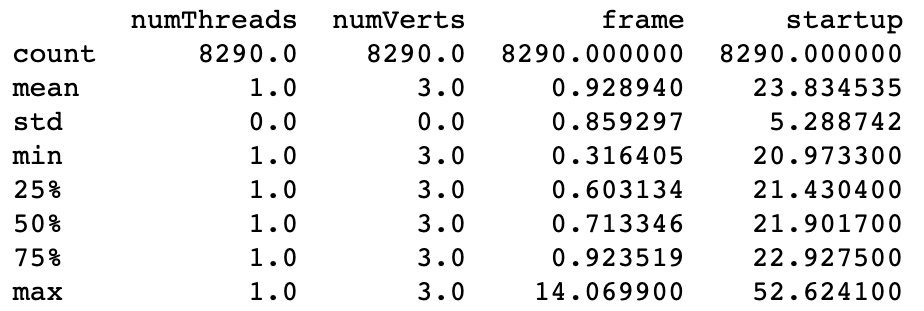
\includegraphics[width=0.9\textwidth]{images/simple_describe.png}
            \caption{Simple triangle.}
          \end{subfigure}
          \begin{subfigure}[b]{0.5\textwidth}
            \centering
            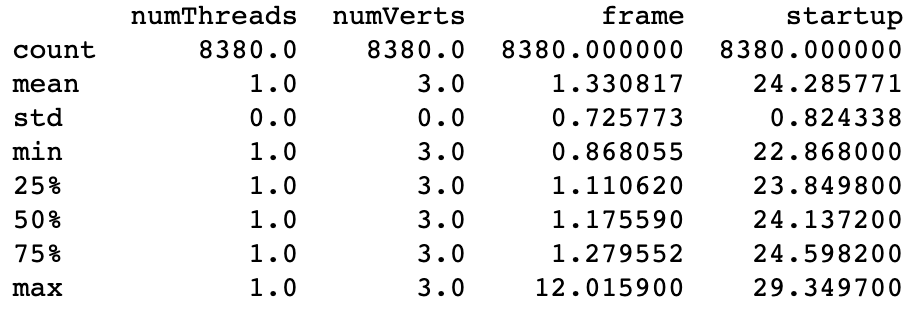
\includegraphics[width=0.9\textwidth]{images/evk_describe.png}
            \caption{evulkan triangle.}
          \end{subfigure}
          \caption{Test results for simple and evulkan triangles.}
          \label{fig:test_describe}                        
        \end{figure}

        The median (50\%) frame draw time for the evulkan Triangle is 0.4ms
        longer than that for the simple triangle, however the evulkan frame
        draw time has a shorter tail for the maximum value.  The same is true
        for the startup time. While the draw and startup times might be
        slightly longer, they are much more consistent - the standard
        deviation of the Simple Triangle is 5.289 while that of the evulkan
        Triangle is 0.824. \\

        Note that the data has been stripped of outlier values (z value larger than 3).
        The Python code used to generate these results is in examples/bench/Bench.ipynb.

    \subsection{Usability}

      This is the main goal of the project. Usability refers to how well a person
      can use the library effectively. Usability here is measured in
      documentation, consistency and lines of code. \\

      The code is fully documented with class and method comments. The
      instructions for how to download, build, install and use the library
      are available in this document. The code itself uses consistent naming
      schemes for methods and variables and is consistent with other open source
      projects, as it uses CMake for distribution and building. The code
      adheres to the Google Style Guide, has maximum 80 character length
      lines and it has const and noexcept methods where possible. Using
      the triangle example for comparison, the pure Vulkan implementation
      uses approximately 914 lines of code, while the evulkan implementation
      uses 94, almost a 10x decrease. 

    \subsection{Availability}

      Availability refers to how easily the code is retrieved. The code is
      available on GitHub, and is structured in the standard open-source
      manner. It has examples and the full source code available for
      distributing and building using CMake.

  \chapter{Conclusion}

    This project is a success, resulting in an easy-to-use Vulkan library,
    removing much of the redundant and repetitive coding from the user
    while still allowing them access to many common Vulkan features.

    \section{What Could Have Been Better}

     \subsection{COVID-19}

      Had COVID-19 not been an issue, given access to the lab machines with
      Linux and Windows, the library could have been tested across different
      configurations. In addition, it would have been useful to have my
      classmates test the program and see if they could write a Vulkan
      program in a limited time frame.

    \subsection{Data-Driven Design}

      While care was taken to ensure this library was designed in a data-friendly
      manner, much of the time spent was ensuring that the library was easy to
      use and understand. These two approaches often are in conflict, ease of
      use was paramount, leaving some cases where the solution is less-than
      optimal in terms of data access and overall speed. Starting off the
      project with a better understanding of Vulkan and library writing
      would have made this step much easier and more fluid.

    \subsection{Mesh Shader}

      There are some new features that would be interesting to integrate with
      the library, specifically mesh shaders. However, the laptop on which
      the library was developed is relatively old (2015 MacBook Pro) and,
      as a result, has a relatively old GPU (Intel Iris Graphics 6100).
      Without a machine on which these new features can be tested, it
      is impossible to ensure a feature is correctly integrated.

  \section{Future Developments}
    
    Possible future developments include exposing more Vulkan features
    (e.g. compute pipeline), adding more tests and integrating it with
    NGL.

  \section{Alternatives Considered}

    \subsection{Bazel}

      There were two options for the build system, Bazel and CMake. Bazel is
      Google's build system. Tests undertaken at the beginning of the
      project found that, while Bazel is good for large codebases and
      modeling interdependencies within the codebase, CMake is the
      standard used for distributing, building and installing
      open-source code across multiple systems.

    \subsection{Node-Based Graph}

      Instead of having a \cpp{} library, an option was to create a node-based visual
      library, similar to how Houdini works. The advantages of this include an
      easier interface for users. \\

      However, this requires using a library to generate the graphs themselves
      as this is not a trivial exercise. Two open-source solutions were
      found online, but one of them was failing its build tests. The
      other (passing) library was an option. However, the author
      decided to focus on the full testing, documentation and
      completion of a stable and usable \cpp{} library. Graphics
      programmers are expected to have a solid understanding
      of \cpp{} so it is safe to assume that they would be able
      to set up and use a simple library such as this one.

  \bibliographystyle{harvardnat}
  \bibliography{thesis.bib}

  \chapter*{Appendices}

    \afterpage
    {
      \begin{figure}
        \begin{subfigure}[b]{\textwidth}
          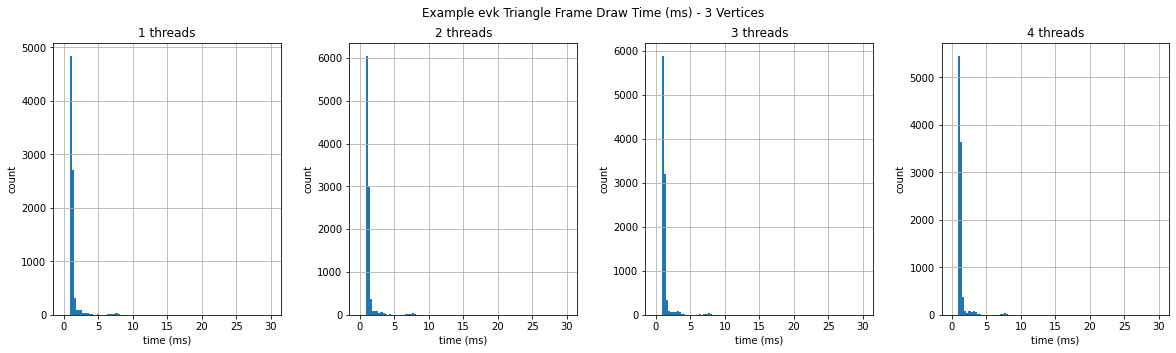
\includegraphics[width=\textwidth]{images/triangle_draw.png}
        \end{subfigure}
        \begin{subfigure}[b]{\textwidth}
          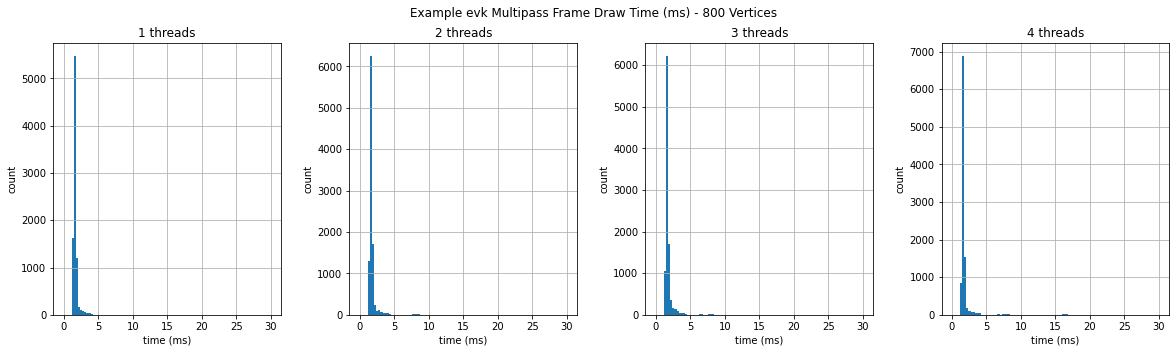
\includegraphics[width=\textwidth]{images/multipass_draw.png}
        \end{subfigure}
        \begin{subfigure}[b]{\textwidth}
          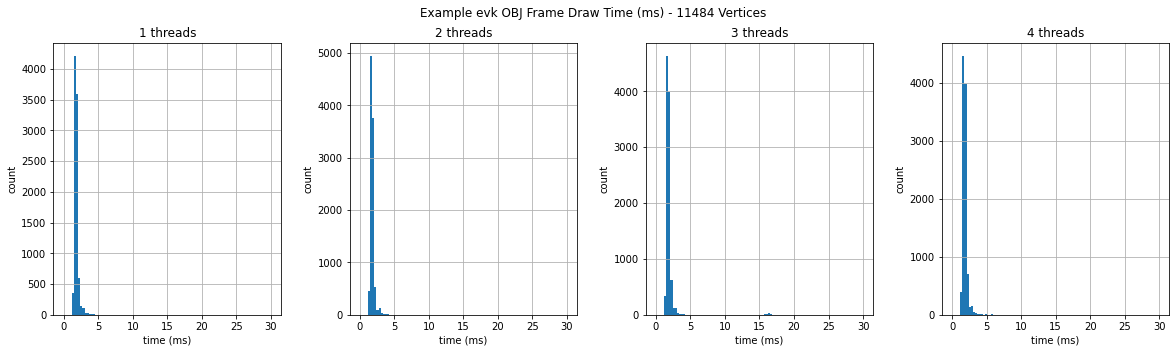
\includegraphics[width=\textwidth]{images/obj_draw.png}
        \end{subfigure}
        \caption{Draw time for different examples over multiple threads.}
        \label{fig:draw}                        
      \end{figure}

      \clearpage

      \begin{figure}
        \begin{subfigure}[b]{\textwidth}
          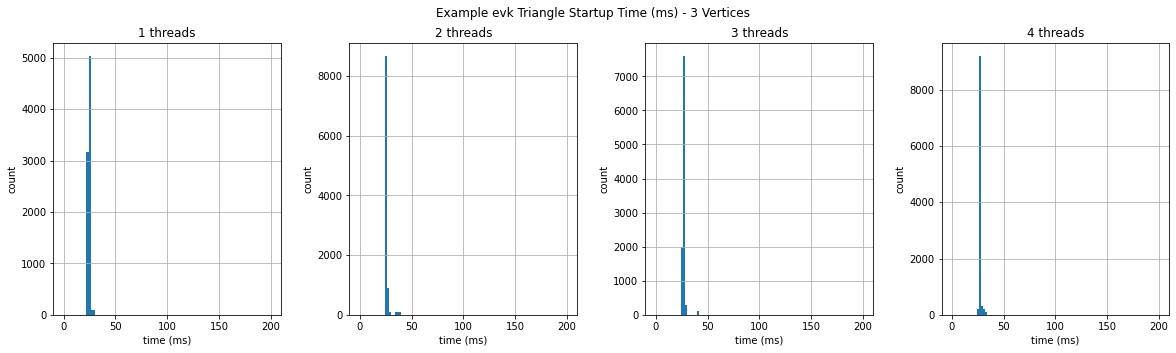
\includegraphics[width=\textwidth]{images/triangle_setup.png}
        \end{subfigure}
        \begin{subfigure}[b]{\textwidth}
          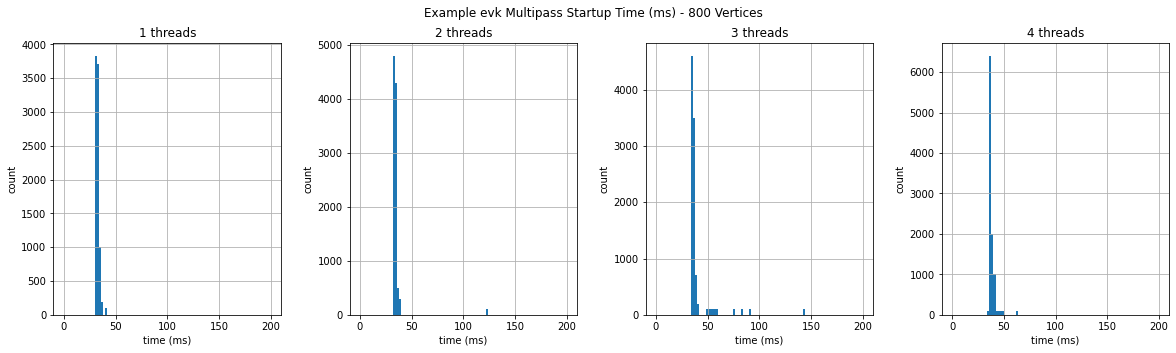
\includegraphics[width=\textwidth]{images/multipass_setup.png}
        \end{subfigure}
        \begin{subfigure}[b]{\textwidth}
          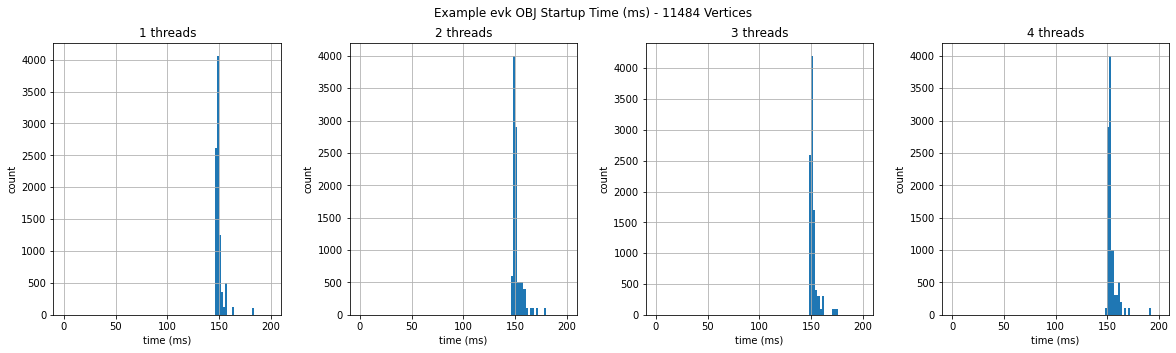
\includegraphics[width=\textwidth]{images/obj_setup.png}
        \end{subfigure}
        \caption{Setup time for different examples over multiple threads.}
        \label{fig:setup}                        
      \end{figure}
      
      \clearpage
    }
  
\end{document}